%%%%%%%%%%%%%%%%%%%%%%%%%%%%%%%%%%%%%%%%%%%%%%%%%%%%%%%%%%%%%%%%%%%%%%%%%%%

\documentclass[a4paper,oneside,12pt]{article}
\usepackage{mystyle}

\begin{document}

\title{\Large\bf Roots of quadratic functions}
\author{%%
  Minh Van Nguyen \\
  \url{mvngu@gmx.com}
}
\date{\today}
\maketitle

\noindent
This document will show you various ways to determine the roots of a
quadratic function.  You already know that the quadratic formula can
be used to determine the roots of any quadratic function.  The purpose
of this document is to show you how to determine the roots
\emph{without} using the quadratic formula.  Why would you want to
learn another technique to find the roots?  One reason is that so you
can check your results.  If using two different techniques produce the
same roots of a quadratic function, then you can be sure that your
results are correct.  Another reason is that in some cases you might
find it easier to use a technique other than the quadratic formula.
In the rest of the document, you will encounter cases where it would
be much easier to factorise a quadratic function than to use the
quadratic formula.  How would you factorise a quadratic function?


%%%%%%%%%%%%%%%%%%%%%%%%%%%%%%%%%%%%%%%%%%%%%%%%%%%%%%%%%%%%%%%%%%%%%%%%%%%

\section{Factoring when $c = 0$}

To factorise an expression means to write the expression as the
product of two or more expressions.  In the case of the number $6$,
you can factorise $6$ by writing it as the product of $2$ and $3$.
Hence the integer $6$ can be written in factored form as
\[
6
=
2 \times 3
\]
and you say that $2$ and $3$ are factors of $6$.  As another example,
you can write $60$ in factored form as $60 = 3 \times 20$.  You can
also factorise $20$ to get $20 = 4 \times 5$ and therefore $60$ can be
factorised as
\[
60
=
3 \times 4 \times 5.
\]
As can be seen from the above examples, factorising an integer
involves writing the integer as the product of two or more integers.
The factors are usually prime integers.  A factorisation such as
$5 = 1 \times 5$ is correct because $5$ is a prime and has no positive
factors other than $1$ and $5$.  The factored form
$5 = 1 \times 5 \times 1$ is also correct, but that's cheating.

What about factoring quadratic functions?  Let's start with quadratic
functions of the form $f(x) = ax^2 + bx$, where $a$ and $b$ are any
real numbers such that $a \neq 0$.  Note that $c = 0$ and so the
vertical intercept of $f(x)$ is the point $\tuple{0}{0}$.  Use the
distributive laws to write $f(x)$ in the factored form
%%
\begin{equation}
\label{eqn:factorise_axx_bx}
f(x)
=
(ax + b)x
\end{equation}
%%
and you can see that $f(x)$ has the factors $x$ and $ax + b$.  Looking
at the factored form~\eqref{eqn:factorise_axx_bx}, the roots of $f(x)$
are $x = 0$ and $x = -b/a$.  But how did you get those numbers?  To
calculate the roots of $f(x)$ means to determine all values of $x$
such that the expression $f(x) = 0$ is true.  In other words, you want
to determine all values of $x$ such that the expression
%%
\begin{equation}
\label{eqn:roots_of_axx_bx}
(ax + b)x
=
0
\end{equation}
%%
is true.  Expression~\eqref{eqn:roots_of_axx_bx} tells you that there
are two numbers, i.e.~$x$ and $ax + b$, whose product is zero.  You
have two cases:
%%
\begin{packedenumeral}
\item If $x = 0$, then \Expression{eqn:roots_of_axx_bx} is true
  because zero multiplied by another number is zero.  So one root of
  $f(x)$ is $x = 0$.

\item If $ax + b = 0$, then \Expression{eqn:roots_of_axx_bx} is also
  true.  But for which values of $x$ would you have $ax + b = 0$?
  Solving the latter expression for $x$ shows that $x = -b / a$.
  Substituting the last expresssion into~\eqref{eqn:roots_of_axx_bx}
  produces
  %%
  \begin{align*}
  \squarebracket*{
    a \parenthesis*{-\frac{b}{a}}
    +
    b
  }
  \parenthesis*{-\frac{b}{a}}
  &=
  (-b + b)
  \parenthesis*{-\frac{b}{a}} \\[4pt]
  &=
  0 \times \parenthesis*{-\frac{b}{a}} \\[4pt]
  &=
  0
  \end{align*}
  %%
  which is true.  Hence you have found that $x = -b / a$ is another
  root of $f(x)$.
\end{packedenumeral}
%%
By writing $f(x)$ as the factored form~\eqref{eqn:factorise_axx_bx}
you can easily determine the roots of $f(x)$ without using the
quadratic formula.  The above discussion is summarised in the
following theorem.

\begin{theorem}
\label{thm:quadratic_function_vertical_intercept_zero}
\textbf{Factorisation.}
Consider the quadratic function $f(x) = ax^2 + bx$, where $a$ and $b$
are any real numbers such that $a \neq 0$.  The roots of $f(x)$ are
\[
x = 0
%%
\qquad
\text{and}
\qquad
%%
x = -\frac{b}{a}.
\]
\end{theorem}

\begin{example}
\label{eg:AmazingCar}
\textbf{AmazingCar.}
At a particular toy store, the sales of a toy called AmazingCar is
given by the sales function $S(x) = -3x + 40$.  Here $x$ represents
the price in dollars of each unit of AmazingCar and so $x$ is the unit
price.  The sales function $S(x)$ represents the number of units of
AmazingCar sold during a week.
%%
\begin{packedenum}
\item\label{subeg:AmazingCar_graph_sales_function}
  Produce a graph of the sales function.  Use the graph to help you
  explain the sales function.  Identify the unit prices at which the
  number of units of AmazingCar sold is highest and lowest.

\item\label{subeg:AmazingCar_revenue_function}
  Derive an expression for the revenue from selling units of
  AmazingCar during a particular week.  Produce a graph of the revenue
  function.

\item\label{subeg:AmazingCar_price_zero_revenue}
  At which unit prices would the revenue from selling units of
  AmazingCar be zero dollars during a week?
\end{packedenum}
\end{example}

\begin{solution}
\solutionpart{subeg:AmazingCar_graph_sales_function}
\Figure{fig:AmazingCar_sales} shows a graph of the sales function
$S(x)$.  The graph shows that as the price for each unit of AmazingCar
increases the lower is the number of units sold during a week.  In
other words, the lower is the unit price the higher is the number of
units sold during the week.  This sounds reasonable because as the
price of something decreases you would expect to sell more of the
product.  Note the two points on the graph that show the lowest and
highest number of units sold.  These are the intercepts of the axes.
The horizontal intercept is the point $\tuple{\frac{40}{3}}{0}$, which
tells you that when the unit price is approximately $\$13.33$ zero
units of AmazingCar would be sold per week.  The lowest number of
units sold per week is zero.  The vertical intercept $\tuple{0}{40}$
tells you that when the unit price is zero dollars~(each unit of
AmazingCar is given away free of charge), the number of units sold per
week is $40$, which is also the highest number of units sold per
week.

\begin{figure}[!htbp]
\centering
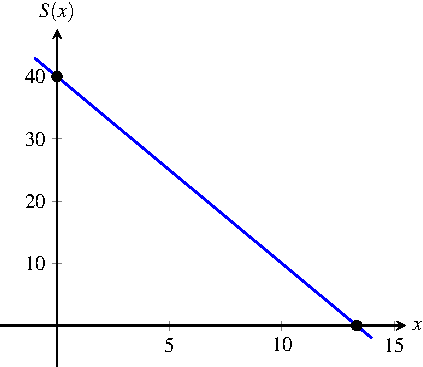
\includegraphics[scale=1.1]{image/10/amazingcar-sales.pdf}
\caption{%%
  Graph of the sales function $S(x) = -3x + 40$ for AmazingCar.  Here
  $x$ represents the unit price in Australian dollars and $S(x)$
  represents the number of units of AmazingCar sold at $x$ dollars
  per unit.
}
\label{fig:AmazingCar_sales}
\end{figure}

\solutionpart{subeg:AmazingCar_revenue_function}
Since $x$ is the unit price and $S(x)$ represents how many units were
sold during a week, the revenue from selling AmazingCar is the
expression
\[
R(x)
=
x S(x)
=
x(-3x + 40).
\]
The revenue function is graphed in \Figure{fig:AmazingCar_revenue}.

\begin{figure}[!htbp]
\centering
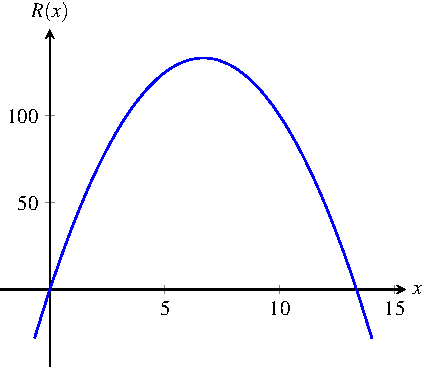
\includegraphics[scale=1.1]{image/10/amazingcar-revenue.pdf}
\caption{%%
  Graph of the revenue function $R(x) = x(-3x + 40)$ for AmazingCar.
  The function $R(x)$ represents the revenue~(in dollars) from selling
  units of AmazingCar during a week at $x$ dollars per unit.
}
\label{fig:AmazingCar_revenue}
\end{figure}

\solutionpart{subeg:AmazingCar_price_zero_revenue}
\Figure{fig:AmazingCar_revenue} shows that you have two unit prices at
which the revenue from selling AmazingCar would be zero dollars during
a week.  Those particular two unit prices are the roots of $R(x)$.
You can use the quadratic formula to determine the roots of $R(x)$.
However, note that you can use the distributive laws to write the
revenue function as
%%
\begin{equation}
\label{eqn:AmazingCar_revenue_function_distributive}
R(x)
=
-3x^2 + 40x.
\end{equation}
%%
You then use \Theorem{thm:quadratic_function_vertical_intercept_zero}
to conclude that the roots of $R(x)$ are $x = 0$ and
\[
x
=
-\frac{40}{-3}
=
\frac{40}{3}.
\]
In other words, the revenue during a week from selling units of
AmazingCar would be zero dollars if the unit prices were either zero
dollars or approximately $\$13.33$.
\end{solution}

\begin{exercise}
\textbf{More AmazingCar.}
You will further explore \Example{eg:AmazingCar}.
%%
\begin{packedenum}
\item\label{subeg:AmazingCar_roots_quadratic_formula}
  Use the quadratic formula to verify the roots of the revenue
  function.

\item\label{subeg:AmazingCar_maximum_revenue}
  Determine the unit price that would result in maximum revenue for a
  week from selling units of AmazingCar.
\end{packedenum}
\end{exercise}

\ifbool{showSolution}{
\begin{solution}
\solutionpart{subeg:AmazingCar_roots_quadratic_formula}
Apply the quadratic formula on the revenue
function~\eqref{eqn:AmazingCar_revenue_function_distributive} to see
that the roots of $R(x)$ are given by the expression
%%
\begin{align*}
x
&=
\frac{
  -40 \pm \sqrt{40^2 - 4(-3)(0)}
}{
  2(-3)
} \\[4pt]
&=
\frac{
  -40 \pm 40
}{
  -6
}.
\end{align*}
Thus the roots of $R(x)$ are
\[
x
=
\frac{-40 + 40}{-6}
=
0
\]
and
\[
x
=
\frac{-40 - 40}{-6}
=
\frac{40}{3}
\]
which are the same as what you got in \Example{eg:AmazingCar}.

\solutionpart{subeg:AmazingCar_maximum_revenue}
The maximum revenue is located at the vertex in the graph of $R(x)$.
The horizontal coordinate of the vertex is
\[
x
=
\frac{-40}{2(-3)}
=
\frac{20}{3}.
\]
The vertical coordinate of the vertex is
\[
R(20/3)
=
\frac{20}{3}
\parenthesis*{
  -3 \times \frac{20}{3}
  +
  40
}
=
\frac{20}{3}
(-20 + 40)
=
\frac{400}{3}.
\]
That is, the maximum revenue for a week from selling units of
AmazingCar would be approximately $\$133.33$, which would occur if the
unit price is approximately $\$6.67$.  All numbers have been rounded
to two decimal places.
\end{solution}
}{}

\begin{exercise}
Consider the function $f(x) = 5x^2 - 3x$.
%%
\begin{packedenum}
\item\label{subex:factorise_a5_bminus3_c0}
  Factorise the function  and determine its roots.

\item\label{subex:verify_roots_substitution_a5_bminus3_c0}
  Verify the roots by substituting the roots into $f(x)$ and simplify.

\item\label{subex:verify_roots_quadratic_formula_a5_bminus3_c0}
  Verify the roots by using the quadratic formula.
\end{packedenum}
\end{exercise}

\ifbool{showSolution}{
\begin{solution}
\solutionpart{subex:factorise_a5_bminus3_c0}
For the function $f(x) = 5x^2 - 3x$, you can use the distributive laws
to factor out the $x$ and you get
\[
f(x)
=
x(5x - 3).
\]
As for the roots of $f(x)$, you now set $f(x)$ to zero and determine
for which values of $x$ would the expression $f(x) = 0$ be true.  In
other words, you want all values of $x$ such that the expression
$x(5x - 3) = 0$ is true.  The latter expression is true when $x = 0$
because $0 \times (5x - 3)$ becomes zero.  So one root of $f(x)$
occurs at $x = 0$.  If $5x - 3 = 0$, then $x \times 0 = 0$ is also
true.  The expression $5x - 3 = 0$ can also be written as $5x = 3$ and
solving for $x$ produces $x = 3 / 5$, which is another root of
$f(x)$.  Therefore the roots of $f(x)$ are $x = 0$ and $x = 3 / 5$.

\solutionpart{subex:verify_roots_substitution_a5_bminus3_c0}
Let's check your results by substitution.  If you substitute each root
into $f(x)$ and simplify, you should get zero as a function value.
Substitute the root $x = 0$ into $f(x)$ and simplify to get
\[
f(0)
=
5(0^2) - 3(0)
=
0.
\]
Now substitute $x = 3 / 5$ into $f(x)$ and simplify to get
%%
\begin{align*}
f(3 / 5)
&=
5\parenthesis*{\frac{3}{5}}^2
-
3\parenthesis*{\frac{3}{5}} \\[4pt]
&=
5 \times \frac{3}{5} \times \frac{3}{5}
-
3 \times \frac{3}{5} \\[4pt]
&=
3 \times \frac{3}{5}
-
3 \times \frac{3}{5} \\[4pt]
&=
0
\end{align*}
%%
as required.

\solutionpart{subex:verify_roots_quadratic_formula_a5_bminus3_c0}
The quadratic formula shows that the roots of $f(x)$ are
%%
\begin{align*}
x
&=
\frac{
  -(-3)
  \pm
  \sqrt{
    (-3)^2 - 4(5)(0)
  }
}{
  2(5)
} \\[4pt]
&=
\frac{
  3
  \pm
  \sqrt{9}
}{
  10
} \\[4pt]
&=
\frac{3 \pm 3}{10}.
\end{align*}
%%
Thus one root of $f(x)$ is
\[
x_1
=
\frac{3 + 3}{10}
=
\frac{6}{10}
=
\frac{3}{5}
\]
and the other root is
\[
x_2
=
\frac{3 - 3}{10}
=
\frac{0}{10}
=
0.
\]
These are the same as the roots you obtained
in \Part{subex:factorise_a5_bminus3_c0}.
\end{solution}
}{}


%%%%%%%%%%%%%%%%%%%%%%%%%%%%%%%%%%%%%%%%%%%%%%%%%%%%%%%%%%%%%%%%%%%%%%%%%%%

\section{Factoring when $a = 1$}
\label{sec:factor_quadratic_a_1}

Given the quadratic function $f(x) = ax^2 + bx + c$, if $a = 1$ then
the function simplifies to the expression
%%
\begin{equation}
\label{eqn:monic_quadratic_function}
f(x)
=
x^2 + bx + c
\end{equation}
%%
You have already seen examples of this function, especially when you
were considering the interpretation of a quadratic function as the
area of a rectangle.  This interpretation is illustrated in
\Figure{fig:quadratic_as_rectangle}, which you have seen before.  From
the figure, you can write the area of the larger rectangle as the
expression
%%
\begin{equation}
\label{eqn:monic_quadratic_function_factored}
(x + \alpha) (x + \beta)
=
x^2 + (\alpha + \beta)x + \alpha\beta.
\end{equation}
%%
How is \Expression{eqn:monic_quadratic_function_factored} related to
the problem of factoring a quadratic function?

\begin{figure}[!htbp]
\centering
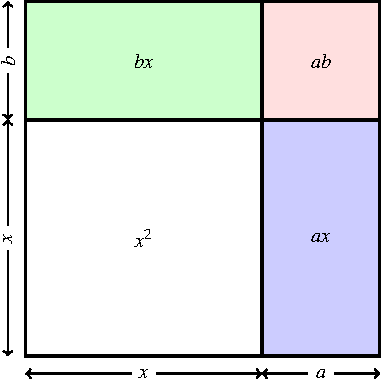
\includegraphics[scale=1.1]{image/08/quadratic-as-square.pdf}
\caption{%%
  The quadratic function $f(x) = (x + \alpha)(x + \beta)$ can be
  interpreted as a rectangle whose base and height have lengths
  $x + \alpha$ and $x + \beta$, respectively.
}
\label{fig:quadratic_as_rectangle}
\end{figure}

The obvious answer is that
\Expression{eqn:monic_quadratic_function_factored} gives you the
factored form of the quadratic function
%%
\begin{equation}
\label{eqn:monic_quadratic_function_roots}
f(x)
=
x^2 + (\alpha + \beta)x + \alpha\beta.
\end{equation}
%%
One factor is $x + \alpha$, the other factor is $x + \beta$, and
therefore the roots of $f(x)$ are $x = -\alpha$ and $x = -\beta$.  In
other words, when you have a quadratic function that can be written as
in \Expression{eqn:monic_quadratic_function}, you ask yourself: How do
I factorise the function so that I end up with something like
expressions~\eqref{eqn:monic_quadratic_function_factored}
or~\eqref{eqn:monic_quadratic_function_roots}?  If you compare
\Expressions{eqn:monic_quadratic_function}{eqn:monic_quadratic_function_factored},
you will notice that you have two equations:
%%
\begin{equation}
\label{eqn:monic_quadratic_function_factors_sum_product}
\alpha + \beta
=
b
%%
\qquad
\text{and}
\qquad
%%
\alpha\beta
=
c.
\end{equation}
%%
These equations tell you that you want two numbers $\alpha$ and
$\beta$ such that when they are added together you get $b$ and when
they are multiplied together you get $c$.  The problem now is to
determine the values of $\alpha$ and $\beta$.  The examples below will
help to clarify the theory.  The above discussion is summarised in the
next theorem.

\begin{theorem}
\textbf{Factorisation.}
Consider the quadratic function
$f(x) = x^2 + (\alpha + \beta)x + \alpha\beta$, where $\alpha$ and
$\beta$ are any real numbers.  Then $f(x)$ can be written in factored
form as $f(x) = (x + \alpha) (x + \beta)$ and the roots of $f(x)$ are
$x = -\alpha$ and $x = -\beta$.
\end{theorem}

\begin{example}
\label{eg:factorise_monic_a1_b2_c6}
Consider the function $f(x) = x^2 + 5x + 6$.  Factorise $f(x)$ and
determine its roots.  Check your results by using the quadratic
formula.
\end{example}

\begin{solution}
The function $f(x)$ has the form similar to
\Expression{eqn:monic_quadratic_function} so you should consider the
equations
in~\eqref{eqn:monic_quadratic_function_factors_sum_product}.  That is,
you want two numbers whose sum is $5$ and whose product is $6$.  You
need to know the integer factors of $6$.  The positive factors of $6$
are $1$, $2$, $3$, and $6$.  The negative factors are obtained by
multiplying each positive factor by $-1$.  Then the integer factors of
$6$ are
\[
\octuple{1}{2}{3}{6}{-1}{-2}{-3}{-6}.
\]
Among these factors, choose two that sum to $5$ and have a product of
$6$.  The required factors are $2$ and $3$ because $2 + 3 = 5$ and
$2 \times 3 = 6$.  Thus $f(x)$ can be written in factored form as
$f(x) = (x + 2) (x + 3)$.  If $x = -2$, then $f(-2)$ simplifies to
zero.  If $x = -3$, then $f(-3)$ also becomes zero.  Therefore the
roots of $f(x)$ are $x = -2$ and $x = -3$.

You can verify the roots you obtained above by using the quadratic
formula.  The quadratic formula shows that the roots of $f(x)$ are
%%
\begin{align*}
x
&=
\frac{
  -5
  \pm
  \sqrt{
    5^2 - 4(1)(6)
  }
}{
  2(1)
} \\[4pt]
&=
\frac{
  -5
  \pm
  \sqrt{
    25 - 24
  }
}{
  2
} \\[4pt]
&=
\frac{
  -5 \pm 1
}{
  2
}.
\end{align*}
%%
Then one root of $f(x)$ is
\[
x_1
=
\frac{-5 + 1}{2}
=
\frac{-4}{2}
=
-2
\]
and the other root is
\[
x_2
=
\frac{-5 - 1}{2}
=
\frac{-6}{2}
=
-3.
\]
These are the same roots as obtained above.
\end{solution}

\begin{exercise}
Factorise the function $f(x) = x^2 + 7x + 12$ and determine its
roots.  Use the quadratic formula to verify your results.
\end{exercise}

\ifbool{showSolution}{
\begin{solution}
You want two numbers that sum to $7$ and have a product of $12$.  The
integer factors of $12$ are
\[
\sextuple{1}{2}{3}{4}{6}{12}
\]
among which $3$ and $4$ are the required integers.  Thus you have the
factored form $f(x) = (x + 3) (x + 4)$.  If $x = -3$, then $f(-3)$
simplifies to zero.  If $x = -4$, then $f(-4)$ also becomes zero.
Therefore the roots of $f(x)$ are $x = -3$ and $x = -4$.

Now use the quadratic formula to verify the roots that you obtained
above.  The quadratic formula shows that the roots of $f(x)$ are
%%
\begin{align*}
x
&=
\frac{
  -7
  \pm
  \sqrt{
    7^2 - 4(1)(12)
  }
}{
  2(1)
} \\[4pt]
&=
\frac{
  -7
  \pm
  \sqrt{
    49 - 48
  }
}{
  2
} \\[4pt]
&=
\frac{
  -7 \pm 1
}{
  2
}.
\end{align*}
%%
Thus one root of $f(x)$ is
\[
x_1
=
\frac{-7 + 1}{2}
=
\frac{-6}{2}
=
-3
\]
and the other root is
\[
x_2
=
\frac{-7 - 1}{2}
=
\frac{-8}{2}
=
-4.
\]
These are the same roots as obtained above.
\end{solution}
}{}

\begin{example}
Consider the function $g(x) = 2x^2 + 16x + 30$.  Factorise the
function and determine its roots.  Use the quadratic formula to verify
your results.
\end{example}

\begin{solution}
The function $g(x)$ looks like it is different from
\Expression{eqn:monic_quadratic_function}, but not really.  The trick
is to write $g(x)$ in such a way that allows you to use the technique
explained in \Example{eg:factorise_monic_a1_b2_c6}.  Note that each of
the three terms in $g(x)$ has a common factor, namely $2$.  Factoring
out the $2$ and $g(x)$ can be written as
%%
\begin{align*}
g(x)
&=
2 (x^2 + 8x + 15) \\[4pt]
&=
2 \cdot h(x)
\end{align*}
%%
where $h(x) = x^2 + 8x + 15$.  Note that the roots of $h(x)$ are also
the roots of $g(x)$.  The reason is that if $x = x_1$ is any root of
$h(x)$, then $h(x_1)$ simplifies to zero and hence $2 \cdot h(x_1)$
also becomes zero.  Thus $x_1$ is a root of $g(x)$.  In other words,
you need only to determine the roots of $h(x)$.

Let's factorise $h(x)$.  The function $h(x)$ has a form similar to
\Expression{eqn:monic_quadratic_function} so you can use the technique
explained in \Example{eg:factorise_monic_a1_b2_c6} to factorise
$h(x)$.  You want two numbers that add up to $8$ and have a product of
$15$.  The positive integer factors of $15$ are $1$, $3$, $5$, and
$15$.  Multiply each positive factor by $-1$ to get a negative integer
factor.  Then the integer factors of $15$ are
\[
\octuple{1}{3}{5}{15}{-1}{-3}{-5}{-15}.
\]
Among these factors, $3$ and $5$ are the required integers because
$3 + 5 = 8$ and $3 \times 5 = 15$.  Now write $h(x)$ in the factored
form $h(x) = (x + 3) (x + 5)$ and therefore $g(x)$ can be written in
the factored form
\[
g(x)
=
2 (x + 3) (x + 5).
\]
If $x = -3$, then $g(-3)$ simplifies to zero.  If $x = -5$, then
$g(-5)$ also becomes zero.  Therefore the roots of $g(x)$ are
$x = -3$ and $x = -5$.

Now use the quadratic formula to verify the roots that you obtained
above.  The quadratic formula shows that $g(x)$ has the roots
%%
\begin{align*}
x
&=
\frac{
  -16
  \pm
  \sqrt{16^2 - 4(2)(30)}
}{
  2(2)
} \\[4pt]
&=
\frac{
  -16
  \pm
  \sqrt{256 - 240}
}{
  4
} \\[4pt]
&=
\frac{
  -16 \pm 4
}{
  4
}.
\end{align*}
%%
So one root of $g(x)$ is
\[
x_1
=
\frac{-16 + 4}{4}
=
\frac{-12}{4}
=
-3
\]
and the other root is
\[
x_2
=
\frac{-16 - 4}{4}
=
\frac{-20}{4}
=
-5.
\]
These are the same roots as obtained above.
\end{solution}

\begin{exercise}
Factorise the function $g(x) = 3x^2 + 15x + 18$ and determine its
roots.  Use the quadratic formula to check your results.
\end{exercise}

\ifbool{showSolution}{
\begin{solution}
The trick is to write $g(x)$ in a form similar to
\Expression{eqn:monic_quadratic_function}.  Doing so would allow you
to use the technique explained in
\Example{eg:factorise_monic_a1_b2_c6}.  Each of the three terms in
$g(x)$ has $3$ as a common factor.  Factor out the $3$ to write $g(x)$
as
%%
\begin{align*}
g(x)
&=
3 (x^2 + 5x + 6) \\[4pt]
&=
3 \cdot h(x)
\end{align*}
where $h(x) = x^2 + 5x + 6$.  The function $h(x)$ is the same as the
function in \Example{eg:factorise_monic_a1_b2_c6} so you have the
factored form $h(x) = (x + 2) (x + 3)$ and therefore $g(x)$ has the
factored form
\[
g(x)
=
3 (x + 2) (x + 3).
\]
Then the roots of $g(x)$ are the same roots derived in
\Example{eg:factorise_monic_a1_b2_c6}.
\end{solution}
}{}

\begin{example}
\label{eg:factored_form_bminus2_c1}
Factorise $f(x) = x^2 - 2x + 1$ and determine its roots.  Check your
results by means of the quadratic formula.
\end{example}

\begin{solution}
You need to be careful about the negative sign.  The function $f(x)$
has a form similar to \Expression{eqn:monic_quadratic_function}.  You
require two numbers that sum to $-2$ and have a product of $1$.  Since
there is a negative sign, you must consider all integer factors of
$1$, both the positive and negative factors.  The positive factor of
$1$ is $1$ itself.  Now multiply each positive factor by $-1$ to get
the negative factors.  So multiplying $1$ by $-1$ results in $-1$.
Then the factors of $1$ are
\[
\pair{-1}{1}.
\]
The required integers are $-1$ and $-1$ again because you have the sum
\[
(-1) + (-1)
=
-2
\]
and the product $(-1) \times (-1) = 1$.  Now write $f(x)$ in the
factored form
\[
f(x)
=
(x - 1)^2.
\]
If $x = 1$, then $f(1)$ simplifies to zero.  Therefore $f(x)$ has the
root $x = 1$.

Now check your result via the quadratic formula.  Using the quadratic
formula, you have the root
%%
\begin{align*}
x
&=
\frac{
  -(-2)
  \pm
  \sqrt{(-2)^2 - 4(1)(1)}
}{
  2(1)
} \\[4pt]
&=
\frac{
  2
  \pm
  \sqrt{4 - 4}
}{
  2
} \\[4pt]
&=
\frac{
  2 \pm 0
}{
  2
} \\[4pt]
&=
1
\end{align*}
%%
which is the same as what you obtained above.
\end{solution}

\begin{exercise}
Factorise $f(x) = -x^2 + 1$ and determine its roots.  Verify your
results by means of the quadratic formula.
\end{exercise}

\ifbool{showSolution}{
\begin{solution}
Note that the function $f(x)$ can be written as
\[
f(x)
=
-(x^2 - 1)
=
-(x^2 + 0 \cdot x - 1).
\]
If you define the function $g(x) = x^2 + 0 \cdot x - 1$, then $f(x)$
can be written as
\[
f(x)
=
-g(x).
\]
In other words, you need only to determine the roots of $g(x)$.

Let's factorise $g(x)$.  You want two numbers that sum to zero and
have a product of $-1$.  The integer factors of $-1$ are
\[
\pair{-1}{1}.
\]
Among these factors, $-1$ and $1$ are the required numbers because you
have the sum $-1 + 1 = 0$ and the product $(-1) \times 1 = -1$.  Now
write $g(x)$ in the factored form $g(x) = (x - 1) (x + 1)$ and
therefore $f(x)$ can be written in factored form as
\[
f(x)
=
-(x - 1) (x + 1).
\]
If $x = 1$, then $f(1)$ simplifies to zero.  If $x = -1$, then $f(-1)$
also becomes zero.  Therefore the roots of $f(x)$ are $x = -1$ and
$x = 1$.

Finally, you verify your results.  The quadratic formula shows that
the roots of $f(x)$ are
%%
\begin{align*}
x
&=
\frac{
  -0
  \pm
  \sqrt{0^2 - 4(-1)(1)}
}{
  2(-1)
} \\[4pt]
&=
\frac{
  \pm \sqrt{4}
}{
  -2
} \\[4pt]
&=
\frac{\pm 2}{-2}.
\end{align*}
%%
Then one root of $f(x)$ is
\[
x_1
=
\frac{2}{-2}
=
-1
\]
and the other root is
\[
x_2
=
\frac{-2}{-2}
=
1.
\]
These are the same roots as those you obtained above.
\end{solution}
}{}


%%%%%%%%%%%%%%%%%%%%%%%%%%%%%%%%%%%%%%%%%%%%%%%%%%%%%%%%%%%%%%%%%%%%%%%%%%%

\section{Completing the square: special case}
\label{sec:completing_the_square_special_case}

The idea of \emph{completing the square} is to turn a quadratic
function from the form $f(x) = ax^2 + bx + c$ into the form
%%
\begin{equation}
\label{eqn:completing_square_general_form}
f(x)
=
\alpha(x + \beta)^2 + \gamma
\end{equation}
%%
where $\alpha$, $\beta$, and $\gamma$ are numbers that can be written
in terms of $a$, $b$, and $c$.  First, let's consider the case where
$a = 1$.  That is, you want to write
\[
f(x)
=
x^2 + bx + c
\]
in a form similar to \Expression{eqn:completing_square_general_form}.
From \Section{sec:factor_quadratic_a_1} you already know how to
factorise $f(x)$ and determine its roots.  However, let's see how to
determine the roots of $f(x)$ in a different way.  To understand how
this can be accomplished, consider the function $g(x) = x^2 + bx$ so
that you have
%%
\begin{equation}
\label{eqn:completing_square_special_case}
f(x)
=
g(x) + c.
\end{equation}
%%
The function $g(x)$ can be interpreted as the area that results from
adding the area of a square to the area of a rectangle; see
\Figure{fig:special_complete_square_square_plus_rectangle}.  The
square has a side length of $x$ and hence an area of $x^2$.  The
rectangle has a width and height of lengths $b$ and $x$, respectively,
and so an area of $bx$.  At this point, you might ask yourself:  What
about the constant $c$?

\begin{figure}[!htbp]
\centering
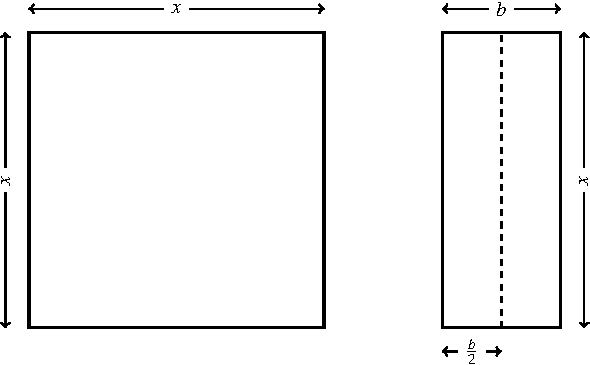
\includegraphics[scale=1.1]{image/10/complete-square-a1-c0.pdf}
\caption{%%
  The quadratic function $g(x) = x^2 + bx$ can be visualised as a
  square plus a rectangle.  The square has a side length of $x$, hence
  the area of the square is $x^2$.  The rectangle has a width of $b$
  and a height of $x$, so the rectangle has an area of $bx$.  Thus
  $g(x)$ can be interpreted as the area of a square plus the area of a
  rectangle.  The rectangle can be cut in half along the dashed line
  as shown.  Each half has a width of $b/2$ and a height of $x$.
}
\label{fig:special_complete_square_square_plus_rectangle}
\end{figure}

\begin{figure}[!htbp]
\centering
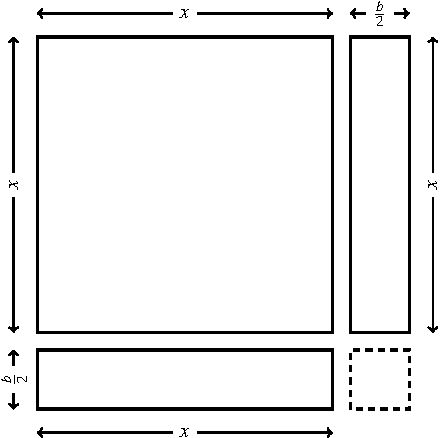
\includegraphics[scale=1.1]{image/10/complete-square-a1-c0_halfb.pdf}
\caption{%%
  The quadratic function $g(x) = x^2 + bx$ can be visualised as a
  square plus a rectangle.  The rectangle is cut in half.  One half is
  arranged to the right of the square.  The other half is arranged
  underneath the square.  Now you have a shape that is nearly like a
  square.  The small dashed square in the lower right is what is
  missing to make a complete square.
}
\label{fig:special_complete_square_nearly_square}
\end{figure}

To see how you can account for the constant $c$, consider cutting the
rectangle in half along the dashed line shown in
\Figure{fig:special_complete_square_square_plus_rectangle}.  Move one
half to the bottom of the square and the other half to the right side
of the square, as shown in
\Figure{fig:special_complete_square_nearly_square}.  What you end up
with is a shape that looks similar to a whole square, except for a
missing small piece in the lower-right corner.  The missing piece is a
square whose side length is $b/2$ and hence the square has an area of
$\parenthesis*{\frac{b}{2}}^2$.  In other words, adding the area
$\parenthesis*{\frac{b}{2}}^2$ to $g(x)$ would result in the area of
the larger square.  Since the larger square has a side length of
$x + \frac{b}{2}$, its area is $\parenthesis*{x + \frac{b}{2}}^2$ and
thus you have the expression
\[
g(x) + \parenthesis*{\frac{b}{2}}^2
=
\parenthesis*{x + \frac{b}{2}}^2
\]
which can be solved for $g(x)$ to produce
\[
g(x)
=
\parenthesis*{x + \frac{b}{2}}^2
-
\parenthesis*{\frac{b}{2}}^2.
\]
Substitute the latter expression
into~\eqref{eqn:completing_square_special_case} and you get
%%
\begin{equation}
\label{eqn:completing_square_special_case_squared}
\begin{aligned}
f(x)
&=
\parenthesis*{x + \frac{b}{2}}^2
-
\parenthesis*{\frac{b}{2}}^2
+
c \\[4pt]
&=
\parenthesis*{x + \frac{b}{2}}^2
+
c
-
\parenthesis*{\frac{b}{2}}^2.
\end{aligned}
\end{equation}
%%
The \Expression{eqn:completing_square_special_case_squared} has a form
that is similar to \Expression{eqn:completing_square_general_form}
because you can make the substitutions
\[
\alpha
=
1,
%%
\qquad
%%
\beta
=
\frac{b}{2},
%%
\qquad
%%
\gamma
=
c
-
\parenthesis*{\frac{b}{2}}^2.
\]

How would you use
\Expression{eqn:completing_square_special_case_squared} to determine
the roots of $f(x)$?  That is, how can
\Expression{eqn:completing_square_special_case_squared} help you to
determine all values of $x$ such that the expression
$f(x) = 0$ is true?  You equate
\Expression{eqn:completing_square_special_case_squared} to zero to get
\[
\parenthesis*{x + \frac{b}{2}}^2
+
c
-
\parenthesis*{\frac{b}{2}}^2
=
0
\]
which can also be written as
\[
\parenthesis*{x + \frac{b}{2}}^2
=
\parenthesis*{\frac{b}{2}}^2 - c.
\]
In the latter expression, taking the square root of both sides results
in
\[
x + \frac{b}{2}
=
\pm
\sqrt{
  \parenthesis*{\frac{b}{2}}^2 - c
}
\]
and solve for $x$ to get the roots
\[
x
=
-\frac{b}{2}
\pm
\sqrt{
  \parenthesis*{\frac{b}{2}}^2 - c
}.
\]
The above discussion is summarised in the next theorem.

\begin{theorem}
\label{thm:monic_quadratic_roots}
\textbf{Completing the square.}
Let $f(x) = x^2 + bx + c$ be a quadratic function, where $b$ and $c$
are given constants.  Then $f(x)$ can be written as
\[
f(x)
=
\parenthesis*{x + \frac{b}{2}}^2
+
c
-
\parenthesis*{\frac{b}{2}}^2
\]
and the roots of $f(x)$ are given by
\[
x
=
-\frac{b}{2}
\pm
\sqrt{
  \parenthesis*{\frac{b}{2}}^2 - c
}.
\]
\end{theorem}

So far so good.  The next question is: How can you use
\Theorem{thm:monic_quadratic_roots} to help you determine the roots of
a quadratic function?

\begin{example}
\label{eg:completing_square_monic_bminus10_c21}
Consider the function $f(x) = x^2 - 10x + 21$.
%%
\begin{packedenum}
\item\label{subeg:completing_square_roots_a1_bminus10_c21}
  Use the technique of completing the square to determine the roots of
  $f(x)$.

\item\label{subeg:completing_square_verify_substitution_a1_bminus10_c21}
  Check your results by substituting the roots into $f(x)$.

\item\label{subeg:completing_square_verify_quadform_a1_bminus10_c21}
  Verify your results by means of the quadratic formula.
\end{packedenum}
\end{example}

\begin{solution}
\solutionpart{subeg:completing_square_roots_a1_bminus10_c21}
You can use the technique explained
in \Section{sec:factor_quadratic_a_1} to factorise $f(x)$ and then
read off its roots.  However, let's see how the roots of $f(x)$ can be
determined by applying \Theorem{thm:monic_quadratic_roots}.  The
function $f(x) = x^2 - 10x + 21$ has a form that is similar to the
general quadratic function in \Theorem{thm:monic_quadratic_roots}
because you have $b = -10$ and $c = 21$.  Use
\Theorem{thm:monic_quadratic_roots} to write $f(x)$ as the expression
%%
\begin{align*}
f(x)
&=
\parenthesis*{x + \frac{-10}{2}}^2
+
21 - \parenthesis*{\frac{-10}{2}}^2 \\[4pt]
&=
(x - 5)^2
+
21 - (-5)^2 \\[4pt]
&=
(x - 5)^2 + 21 - 25 \\[4pt]
&=
(x - 5)^2 - 4.
\end{align*}
%%
The roots of $f(x)$ are all values of $x$ such that the expression
$f(x) = 0$ is true.  That is, you want all values of $x$ such that the
expression
\[
(x - 5)^2 - 4
=
0
\]
is true.  The latter expression can also be written as
$(x - 5)^2 = 4$ and taking the square root of both sides results in
$x - 5 = \pm\sqrt{4}$.  Now solve for $x$ to get the roots
$x = 5 \pm 2$.  Therefore one root of $f(x)$ is $x = 7$ and the other
root is $x = 3$.

\solutionpart{subeg:completing_square_verify_substitution_a1_bminus10_c21}
You can check your results by substituting each root into $f(x)$.
Doing so should produce zero as the function value.  Substituting the
root $x = 7$ into $f(x)$ results in
%%
\begin{align*}
f(7)
&=
7^2 - 10(7) + 21 \\[4pt]
&=
49 - 70 + 21 \\[4pt]
&=
70 - 70 \\[4pt]
&=
0.
\end{align*}
%%
Substitute the root $x = 3$ into $f(x)$ to get
%%
\begin{align*}
f(3)
&=
3^2 - 10(3) + 21 \\[4pt]
&=
9 - 30 + 21 \\[4pt]
&=
30 - 30 \\[4pt]
&=
0
\end{align*}
%%
as required.

\solutionpart{subeg:completing_square_verify_quadform_a1_bminus10_c21}
You can also use the quadratic formula to verify your results.  The
quadratic formula shows that the roots of $f(x)$ are
%%
\begin{align*}
x
&=
\frac{
  -(-10)
  \pm
  \sqrt{(-10)^2 - 4(1)(21)}
}{
  2(1)
} \\[4pt]
&=
\frac{
  10
  \pm
  \sqrt{100 - 84}
}{
  2
} \\[4pt]
&=
\frac{
  10 \pm 4
}{
  2
}.
\end{align*}
%%
One root of $f(x)$ is
\[
x_1
=
\frac{10 + 4}{2}
=
\frac{14}{2}
=
7
\]
and the other root is
\[
x_2
=
\frac{10 - 4}{2}
=
\frac{6}{2}
=
3.
\]
These are the same roots as those you derived
in \Part{subeg:completing_square_roots_a1_bminus10_c21}.
\end{solution}

\begin{exercise}
Repeat \Example{eg:completing_square_monic_bminus10_c21} by using the
technique explained in \Section{sec:factor_quadratic_a_1} to determine
the roots of $f(x) = x^2 - 10x + 21$.
\end{exercise}

\ifbool{showSolution}{
\begin{solution}
You want two numbers that sum to $-10$ and have a product of $21$.
The positive factors of $21$ are $1$, $3$, $7$, and $21$.  Multiply
each factor by $-1$ to get the negative factors of $21$.  Thus all
factors of $21$ are
\[
\octuple{1}{3}{7}{21}{-1}{-3}{-7}{-21}.
\]
Among these factors, the required integers are $-3$ and $-7$ because
you have the sum $(-3) + (-7) = -10$ and and the product
$(-3) \times (-7) = 21$.  Then $f(x)$ can be written in factored form
as $f(x) = (x - 3) (x - 7)$.  If $x = 3$, then $f(3)$ simplifies to
zero.  If $x = 7$, then $f(7)$ also simplifies to zero.  Therefore the
roots of $f(x)$ are $x = 3$ and $x = 7$.  These roots are the same as
those derived in \Example{eg:completing_square_monic_bminus10_c21}.
\end{solution}
}{}

\begin{exercise}
Repeat \Example{eg:factored_form_bminus2_c1} by using
\Theorem{thm:monic_quadratic_roots} to determine the roots of the
function $f(x) = x^2 - 2x + 1$.  Check your results by substituting
the roots into $f(x)$ and simplify.
\end{exercise}

\ifbool{showSolution}{
\begin{solution}
The function $f(x) = x^2 - 2x + 1$ has a form that is similar to the
function in \Theorem{thm:monic_quadratic_roots} because you have
$b = -2$ and $c = 1$.  Use \Theorem{thm:monic_quadratic_roots} to
write $f(x)$ as the expression
%%
\begin{align*}
f(x)
&=
\parenthesis*{x + \frac{-2}{2}}^2
+
1 - \parenthesis*{\frac{-2}{2}}^2 \\[4pt]
&=
(x - 1)^2 + 1 - (-1)^2 \\[4pt]
&=
(x - 1)^2.
\end{align*}
%%
Therefore $f(x)$ has the root $x = 1$.

To check your result, substitute the root $x = 1$ into $f(x)$.  This
should produce a function value of zero.  Substituting $x = 1$ into
$f(x)$ yields
%%
\begin{align*}
f(1)
&=
1^2 - 2(1) + 1 \\[4pt]
&=
1 - 2 + 1 \\[4pt]
&=
2 - 2 \\[4pt]
&=
0
\end{align*}
as required.
\end{solution}
}{}

\begin{exercise}
Consider the function $f(x) = 4x^2 + 12x - 40$.
%%
\begin{packedenum}
\item\label{subeg:monic_quadratic_x2_x5_completing_square}
  Use the technique of completing the square to determine the roots of
  $f(x)$.

\item\label{subeg:monic_quadratic_x2_x5_factored_form}
  Use factorisation~(i.e.~the technique explained
  in \Section{sec:factor_quadratic_a_1}) to determine the roots of
  $f(x)$.

\item\label{subeg:monic_quadratic_x2_x5_quadratic_formula}
  Use the quadratic formula to determine the roots of $f(x)$.
\end{packedenum}
\end{exercise}

\ifbool{showSolution}{
\begin{solution}
\solutionpart{subeg:monic_quadratic_x2_x5_completing_square}
The function $f(x)$ can be written in such a way that it resembles the
function in \Theorem{thm:monic_quadratic_roots}.  Factoring out the
$4$ to get
%%
\begin{align*}
f(x)
&=
4(x^2 + 3x - 10) \\[4pt]
&=
4 g(x)
\end{align*}
%%
where the function $g(x) = x^2 + 3x - 10$ is similar to the function
in \Theorem{thm:monic_quadratic_roots} because you have $b = 3$ and
$c = -10$.  Note that the roots of $g(x)$ are also the roots of
$f(x)$.  The reason is that if $x = x_1$ is a value of $x$ such that
$g(x_1) = 0$, then $4g(x_1)$ is also zero.  That is, you only need to
determine the roots of $g(x)$, which is simpler than the original
definition of $f(x)$.

Use \Theorem{thm:monic_quadratic_roots} to write $g(x)$ as
%%
\begin{equation}
\label{eqn:completed_square_form_b3_cminus10}
\begin{aligned}
g(x)
&=
\parenthesis*{x + \frac{3}{2}}^2
-
10 - \parenthesis*{\frac{3}{2}}^2 \\[4pt]
&=
\parenthesis*{x + \frac{3}{2}}^2
-
10 - \frac{9}{4} \\[4pt]
&=
\parenthesis*{x + \frac{3}{2}}^2
-
\frac{40}{4} - \frac{9}{4} \\[4pt]
&=
\parenthesis*{x + \frac{3}{2}}^2
-
\frac{49}{4}.
\end{aligned}
\end{equation}
%%
Now you determine the roots of $g(x)$.  In other words, you want all
values of $x$ such that the expression $g(x) = 0$ is true.  Equate
\Expression{eqn:completed_square_form_b3_cminus10} to zero to get
\[
\parenthesis*{x + \frac{3}{2}}^2
-
\frac{49}{4}
=
0
\]
which can also be written as
\[
\parenthesis*{x + \frac{3}{2}}^2
=
\frac{49}{4}.
\]
Take the square root of both sides and you have
%%
\begin{align*}
x + \frac{3}{2}
&=
\pm\sqrt{\frac{49}{4}} \\[4pt]
&=
\pm\frac{\sqrt{49}}{\sqrt{4}} \\[4pt]
&=
\pm\frac{7}{2}.
\end{align*}
%%
Solving the latter expression for $x$ produces
\[
x
=
\pm\frac{7}{2} - \frac{3}{2}.
\]
Therefore one root of $f(x)$ is
\[
x
=
\frac{7}{2} - \frac{3}{2}
=
\frac{7 - 3}{2}
=
2
\]
and the other root is
\[
x
=
-\frac{7}{2} - \frac{3}{2}
=
\frac{-7 - 3}{2}
=
-5.
\]

To check your results, substitute the roots into $f(x)$.  This should
produce a function value of zero.  Substitute the root $x = 2$ into
$f(x)$ to get
%%
\begin{align*}
f(2)
&=
4(2^2) + 12(2) - 40 \\[4pt]
&=
16 + 24 - 40 \\[4pt]
&=
40 - 40 \\[4pt]
&=
0.
\end{align*}
%%
Next, substitute the root $x = -5$ into $f(x)$:
%%
\begin{align*}
f(-5)
&=
4(-5)^2 + 12(-5) - 40 \\[4pt]
&=
100 - 60 - 40 \\[4pt]
&=
100 - 100 \\[4pt]
&=
0.
\end{align*}
%%

\solutionpart{subeg:monic_quadratic_x2_x5_factored_form}
Let's use the technique explained
in \Section{sec:factor_quadratic_a_1} to determine the roots of
$f(x)$.  As explained
in \Part{subeg:monic_quadratic_x2_x5_completing_square}, you need only
to determine the roots of the function $g(x) = x^2 + 3x - 10$.  You
require two numbers that sum to $3$ and have a product of $-10$.  The
positive integer factors of $-10$ are $1$, $2$, $5$, and $10$.
Multiply each factor by $-1$ to get the negative factors.  Thus all
integer factors of $-10$ are
\[
\octuple{1}{2}{5}{10}{-1}{-2}{-5}{-10}.
\]
Among these factors, the required numbers are $5$ and $-2$ because
$5 + (-2) = 3$ and $5 \times (-2) = -10$.  Then $f(x)$ can be written
in factored form as
\[
f(x)
=
4(x - 2) (x + 5).
\]
Therefore the roots of $f(x)$ are $x = 2$ and $x = -5$, which are the
same as those
in \Part{subeg:monic_quadratic_x2_x5_completing_square}.
\end{solution}
}{}


%%%%%%%%%%%%%%%%%%%%%%%%%%%%%%%%%%%%%%%%%%%%%%%%%%%%%%%%%%%%%%%%%%%%%%%%%%%

\section{Completing the square: general case}

The general case of completing the square is very similar to the
special case explained
in \Section{sec:completing_the_square_special_case}.  Given a
quadratic function $f(x) = ax^2 + bx + c$, where $a \neq 0$, you can
factor out the $a$ to get
%%
\begin{align*}
f(x)
&=
a
\parenthesis*{
  x^2 + \frac{b}{a}x + \frac{c}{a}
} \\[4pt]
&=
a \cdot g(x)
\end{align*}
%%
where you have the function
\[
g(x)
=
x^2 + \frac{b}{a}x + \frac{c}{a}.
\]
Note that the roots of $g(x)$ are also the roots of $f(x)$.  The
reason is because if $x = x_1$ is a root of $g(x)$, then you get
$g(x_1) = 0$ and thus the expression $a \cdot g(x_1)$ is also zero.
The upshot is that you need only to determine the roots of $g(x)$.  If
$b / a$ and $c / a$ are both integers, you can try to use the
technique explained in \Section{sec:factor_quadratic_a_1} to determine
the roots of $g(x)$.  However, the technique of completing the square
as explained in \Section{sec:completing_the_square_special_case} will
work regardless of whether $b / a$ and $c / a$ are integers.  In
general, you should use the technique of completing the square to
determine the roots of $g(x)$.  To check your work, you can then
use~(if possible) the technique explained
in \Section{sec:factor_quadratic_a_1}, or you can substitute the roots
into $g(x)$ and derive a function value of zero, or you can use the
quadratic formula to see whether you get the same roots.  The examples
below should help to clarify how to use the technique of completing
the square to determine the roots of any quadratic  function.

\begin{example}
\label{eg:completing_square_a3_bminus7_c2}
Use the technique of completing the square to determine the roots of
the function $f(x) = 3x^2 - 7x + 2$.  Check your results.
\end{example}

\begin{solution}
First, you factor out the $3$.  Doing so results in
\[
f(x)
=
3
\parenthesis*{
  x^2 - \frac{7}{3}x + \frac{2}{3}
}.
\]
If you define the function $g(x) = x^2 - \frac{7}{3}x + \frac{2}{3}$,
then you can write
\[
f(x)
=
3 \cdot g(x).
\]
In the last expression, if you want to determine the roots of $f(x)$,
then this is the same as determining the roots of $g(x)$.

Next, you use the technique of completing the square as explained in
\Theorem{thm:monic_quadratic_roots} to determine the roots of $g(x)$.
Use \Theorem{thm:monic_quadratic_roots} to write $g(x)$ as
%%
\begin{align*}
g(x)
&=
\squarebracket*{
  x
  +
  \parenthesis*{-\frac{7}{3}} \times \frac{1}{2}
}^2
+
\frac{2}{3}
-
\squarebracket*{
  \parenthesis*{-\frac{7}{3}} \times \frac{1}{2}
}^2 \\[4pt]
&=
\parenthesis*{
  x
  -
  \frac{7}{6}
}^2
+
\frac{2}{3}
-
\parenthesis*{-\frac{7}{6}}^2 \\[4pt]
&=
\parenthesis*{
  x
  -
  \frac{7}{6}
}^2
+
\frac{2}{3}
-
\frac{49}{36} \\[4pt]
&=
\parenthesis*{
  x
  -
  \frac{7}{6}
}^2
-
\frac{25}{36}.
\end{align*}
%%
The roots of $g(x)$ are all values of $x$ such that the expression
$g(x) = 0$ is true.  In other words, you want to determine all values
of $x$ such that the expression
\[
\parenthesis*{
  x
  -
  \frac{7}{6}
}^2
-
\frac{25}{36}
=
0
\]
is true.  The last expression can also be written as
\[
\parenthesis*{
  x
  -
  \frac{7}{6}
}^2
=
\frac{25}{36}
\]
and taking the square root of both sides results in
\[
x - \frac{7}{6}
=
\pm
\sqrt{\frac{25}{36}}
=
\pm
\frac{5}{6}.
\]
Now solve for $x$ to get the roots
\[
x
=
\frac{7}{6} \pm \frac{5}{6}.
\]
Therefore one root of $g(x)$ is
\[
x_1
=
\frac{7}{6} + \frac{5}{6}
=
\frac{12}{6}
=
2
\]
and the other root is
\[
x_2
=
\frac{7}{6} - \frac{5}{6}
=
\frac{2}{6}
=
\frac{1}{3}.
\]

Finally, you check your results.  You can use the quadratic formula to
see whether you get the same roots.  However, for now you will
substitute the roots of $g(x)$ into $f(x)$ and derive the function
value of zero.  Substituting the root $x_1 = 2$ into $f(x)$ produces
%%
\begin{align*}
f(2)
&=
3(2)^2 - 7(2) + 2 \\[4pt]
&=
12 - 14 + 2 \\[4pt]
&=
14 - 14 \\[4pt]
&=
0.
\end{align*}
%%
Substitute the root $x_2 = 1 / 3$ into $f(x)$ to get
%%
\begin{align*}
f(1/3)
&=
3\parenthesis*{\frac{1}{3}}^2
-
7\parenthesis*{\frac{1}{3}}
+
2 \\[4pt]
&=
\frac{3}{9}
-
\frac{7}{3}
+
2 \\[4pt]
&=
\frac{1}{3}
-
\frac{7}{3}
+
2 \\[4pt]
&=
-\frac{6}{3} + 2 \\[4pt]
&=
-2 + 2 \\[4pt]
&=
0
\end{align*}
%%
as required.
\end{solution}

\begin{exercise}
Use the quadratic formula to verify the roots in
\Example{eg:completing_square_a3_bminus7_c2}.
\end{exercise}

\ifbool{showSolution}{
\begin{solution}
Using the quadratic formula, the roots of $f(x) = 3x^2 - 7x + 2$ are
%%
\begin{align*}
x
&=
\frac{
  -(-7)
  \pm
  \sqrt{
    (-7)^2 - 4(3)(2)
  }
}{
  2(3)
} \\[4pt]
&=
\frac{
  7
  \pm
  \sqrt{
    49 - 24
  }
}{
  6
} \\[4pt]
&=
\frac{
  7
  \pm
  \sqrt{25}
}{
  6
} \\[4pt]
&=
\frac{
  7 \pm 5
}{
  6
}.
\end{align*}
%%
Therefore one root of $f(x)$ is
\[
x_1
=
\frac{7 + 5}{6}
=
\frac{12}{6}
=
2
\]
and the other root is
\[
x_2
=
\frac{7 - 5}{6}
=
\frac{2}{6}
=
\frac{1}{3}.
\]
These are the same roots as obtained in
\Example{eg:completing_square_a3_bminus7_c2}.
\end{solution}
}{}

\end{document}
